\section{Informazioni generali}
\subsection{Descrizione}
SPID, il Sistema Pubblico di Identità Digitale, è la soluzione che permette di accedere a tutti i servizi online della Pubblica Amministrazione con un'unica Identità Digitale (username e password) utilizzabile da computer, tablet e smartphone.
\subsection{Riferimenti Normativi}
Sono state seguite le REGOLE TECNICHE (articolo 4, comma 2, DPCM 24 ottobre 2014).
\\ Sono state seguite anche le regole del sistema previste da SAML v2 per il profilo “Web
Browser SSO”.
\subsection{Funzionamento in breve}
La richiesta di autenticazione SAML può essere inoltrata 
da un Service Provider all’Identity Provider
usando il binding HTTP Redirect o il binding HTTP POST.
\\ La relativa risposta SAML può invece essere inviata
dall’Identity Provider al Service Provider 
solo tramite il binding HTTP POST.

\section{Interfacce Logiche}
Esaminando le interfacce logiche si può capire il funzionamento.
\subsection{Interfacce dell' Identity Provider}
\begin{itemize}
    \item \textbf{IIDPUserInterface}: permette agli utenti l’interazione via web in fase di autenticazione.
    \item \textbf{IAuthnRequest}: permette la ricezione di richieste di autenticazione SAML.
    \item \textbf{IMetadataRetrieve}: permette il reperimento dei SAML metadata dell’Identity Provider.
\end{itemize}
\subsection{Interfacce del Service Provider}
\begin{itemize}
    \item \textbf{IAuthnResponse}: permette la ricezione delle risposte di autenticazione SAML.
    \item \textbf{IMetadataRetrieve}: permette il reperimento dei SAML metadata del Service Provider.
    \item \textbf{IDSResponse}: permette la ricezione delle risposte da parte del Discovery Service.
\end{itemize}

\pagebreak
\section{Schema Funzionamento}
\subsection{Scenario di Interazione in Modalità SSO}
Di seguito è rappresentato il passaggio di autentificazione nel momento in cui si preme sul pulsante SSO e si viene reindirizzati al Service Provider.
\begin{center}
	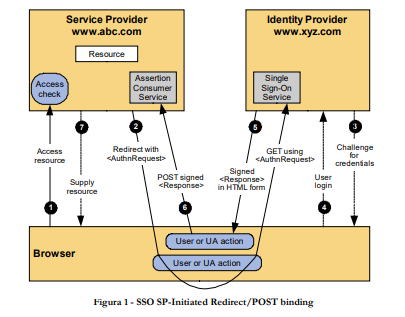
\includegraphics[scale = 1]{./res/images/ScenarioUsoSPIDSchema.PNG}
\end{center}

\section{Scenario Di Utilizzo}
\begin{center}
	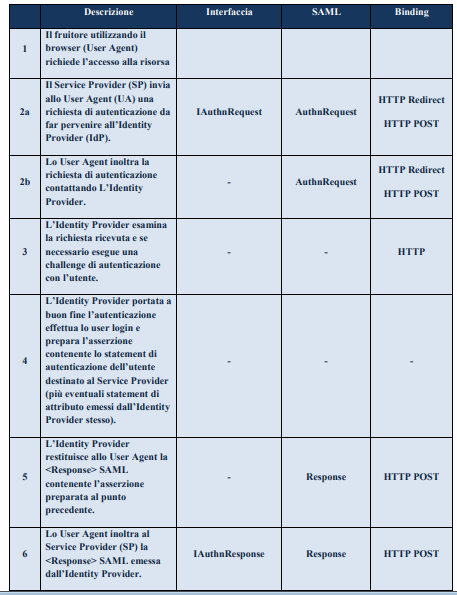
\includegraphics[scale = 1]{./res/images/ScenarioUsoSPID.PNG}
\end{center}

\pagebreak
\section{Binding}
\subsection{Breve descrizione}
Il termine "Binding" si riferisce al momento in cui l'User Agent viene reindirizzato da un portale all'altro durante l'autenticazione. 
In particolare, questo avviene quando il Service Provider reindirizza l'utente all'Identity Provider e, una volta che l'Identity 
Provider ha verificato l'identità dell'utente, lo reindirizza nuovamente al Service Provider per completare il processo\glo di 
autenticazione.
\subsection{Binding HTTP Redirect}
Il Service Provider invia allo User Agent un messaggio HTTP di redirezione, cioè avente uno Status Code con
valore 302 (“Found”) o 303 (“See Other”);
\\ Il Location Header del messaggio HTTP contiene l’URI\glo di destinazione del servizio di Single
Sign-On esposto dall’ Identity Provider.
\\ Il Pacchetto HTTP trasporta i parametri tutti URL-encoded codificato in formato
Base64 e compresso con algoritmo DEFLATE.
\\ Il messaggio all'interno è la risorsa richiesta originaria a cui 
trasferire il controllo una volta terminata l'autenticazione, 
algoritmo e firma per la codifica delle informazioni.
\\ Una volta avute queste informazioni il User Agent fa una 
richiesta GET all' Identity Provider con tutte le informazioni 
sopracitate sotto forma di URLENCODED.

\subsection{Binding HTTP POST}
Il Service Provider invia allo User Agent un messaggio HTTP con uno status code avente valore 200 (“OK”). 
Questo messaggio HTTP contiene un form HTML codificato come valore di un elemento nascosto del form. 
L'utilizzo di questa metodologia consente di superare i limiti di dimensione della query string. \\
L’intero messaggio SAML in formato XML può essere firmato tramite la XML Digital Signature e il risultato viene codificato 
in formato Base64. La risorsa richiesta originariamente è inclusa nel messaggio e viene utilizzata per trasferire il controllo 
a termine dell'autenticazione. Inoltre, è possibile utilizzare un form autopostante attraverso uno script Javascript. \\
Infine, il browser dell’utente elabora la risposta HTTP e invia una richiesta HTTP POST verso il componente Single Sign-On 
dell’Identity Provider.

\section{Invio del Responso}
\subsection{Breve descrizione}
Per Response si intende la risposta che l'Identiry Provider invia al Service Provider con 
l'esito dell'autentificazione e con le informazioni richieste dal Service Provider appartenente all' Utente.
\subsection{Response}
Dopo che l'utente ha completato l'autenticazione, l'Identity Provider crea una Response che contiene la firma digitale e la invia 
direttamente al Service Provider.
\\ La Response viene inclusa in un form HTML come campo nascosto denominato "SAMLResponse". 
\\ L’Identity Provider invia il form HTML al browser dell’utente tramite una risposta
HTTP.
\\ Il browser dell’utente elabora quindi la risposta HTTP e invia una richiesta HTTP POST
contenente la Response firmata verso il Service Provider.

\section{Sicurezza}
\subsection{Accorgimenti Attuati}
Per quanto riguarda la gestione della sicurezza nel canale di trasmissione
si utilizza SSLv.3.0 o TLS 1.0.


\section{Metadata}
\subsection{Scopo}
Ciascuna entità fornisce dei metadati per dichiarare in modo trasparente le proprie caratteristiche, nonché i servizi e le 
informazioni offerti o richiesti.
\subsection{Identity Provider METADATA}
I metadata sono conformi allo standard SAMLv2.0:
\begin{itemize}
    \item \textbf{entityID}: indicante l’identificativo (URI\glo
    ) dell’entità univoco in ambito SPID.
    \item \textbf{Protocollo}: identificatore dei protocolli supportati dall'entità.
    \item \textbf{SingleSignOnService}: endpoint URL del servizio per ricevere le richieste e il tipo di binding da utilizzare con il Service Provider (HTTP-Redirect" oppure HTTP-POST).
    \item \textbf{Organizzazione}: Organizzazione a cui afferisce l'Identity Provider.
    \item \textbf{Signature}: firma proprietaria.
    \item \textbf{Attributi}: uno o più elementi "attribute" ad indicare nome e formato degli attributi certificabili dell’Identity Provider.
    Molto importante, poiché potremmo utilizzare anche noi un sistema simile.
\end{itemize}
I metadata Identity Provider saranno disponibili per tutte le entità SPID federate attraverso
l’interfaccia IMetadataRetrive all'URL "dominioGestoreIdentita/metadata".

\subsection{Service Provider METADATA}

\begin{itemize}
    \item \textbf{IMetadataRetrieve}: permette il reperimento dei SAML metadata del Service Provider da parte dell’Identity Provider.
    \item \textbf{IdentityID}: ID indicante l’identificativo univoco (un URI\glo) dell’entità.
    \item \textbf{Chiave}: chiave pubblica dell'entità per Signature.
    \item \textbf{Signature}: firma proprietaria.
    \item \textbf{AssertionConsumerService}: si riferisce all'indicazione di come il Service Provider deve essere contattato per ricevere la Response, specificando il tipo di binding e l'URI\glo di destinazione.
    \item \textbf{Organizzazione}: organizzazione a cui afferisce il Service Provider.
    \item \textbf{Attributi}: sono una lista di informazioni che il Service Provider richiede all'Identity Provider di fornire, come ad esempio nome, cognome, data di nascita e indirizzo. La lista degli attributi richiesti può variare a seconda del service name desiderato, e possono essere molteplici.
\end{itemize}

\section{Attribute Authority}
\subsection{Descrizione}
Durante la ricerca del sistema SPID non sono state fornite informazioni dettagliate sulle funzioni di questo attore. Tuttavia, è stato chiarito che il suo ruolo è quello di 
verificare gli altri due tipi di enti coinvolti nel sistema.
\\ Esso deve essere in grado di certificare un determinato set di attributi relativi ad un soggetto titolare di
un'identità digitale. 
\\ A fronte di una richiesta di uno o più attributi l’Attribute Authority deve essere
in grado di:
\begin{itemize}
    \item \textbf{1}. ricevere ed interpretare la richiesta di attributo pervenuta da un Service Provider;
    \item \textbf{2}. elaborare la richiesta;
    \item \textbf{3}. costruire la risposta inerente la richiesta pervenuta ed inoltrarla al Service Provider.
\end{itemize}

\subsection{Interfacce}
Il componente Attribute Authority deve esporre le seguenti interfacce:
\begin{itemize}
    \item \textbf{IAttributeQuery}: interfaccia applicativa che supporta le operazioni di richiesta di attributo SAML;
    \item \textbf{IMetadataRetrive}: permette il reperimento dei SAML metadata da parte del Service Provider.
\end{itemize}

\section{Tracciatura Attività}
Le tracce delle attività svolte devono essere conservate nel rispetto delle norme sulla privacy, sotto la responsabilità del 
titolare del trattamento dell'Identity Provider. L'accesso ai dati di tracciatura deve essere consentito solo al personale 
autorizzato. Per tenere traccia delle attività, si utilizza un sistema di gestione di database (DBMS) in cui vengono registrate, 
per un periodo di 24 mesi, le informazioni relative alla richiesta di autenticazione (AuthnRequest) e alla corrispondente risposta 
(Response).

\section{Design e Grafica}
La standardizzazione delle interfacce, della comunicazione e dell'utilizzo del logo SPID è necessaria per gestire l'accesso ai 
servizi pubblici e privati che utilizzano il sistema SPID. Ciò è importante non solo per migliorare l'esperienza dell'utente, 
ma anche per preservare l'immagine del sistema.

\section{SPID Button}
Lo SPID Button consente all'utente la scelta del proprio Identity Provider per l'autenticazione.
Con l'utilizzo di spid-smart-button si intende:
\begin{itemize}
    \item facilitare l'integrazione del bottone "Entra con SPID";
    \item fornire un bottone ospitato via CDN (implementabile tramite javascript e CDN);
    \item migliorare l'esperienza utente.
\end{itemize}


\begin{lstlisting}[style=htmlcssjs]
    //Codice HTML5
    <script type="text/javascript" src="https://XXXXXXXXXXXX/spid-button.min.js"></script>
    <div id="spid-button">
        <noscript> 
            Il login tramite SPID richiede che JavaScript sia abilitato nel browser.
        </noscript>
    </div>
    //Da inizializzare con una chiamata JavaScript
    //Codice Javascript
\end{lstlisting}

\section{Linguaggi di Programmazione e Framework}
E' possibile utilizzare diverse librerie per implementare lo SPID in quasi ogni framework, rendendo l'implementazione del sistema 
indipendente dalla piattaforma. Tra le varie opzioni disponibili, la libreria in PHP sembra essere quella più semplice ed utile. \\
Qui di seguito è disponibile una demo che mostra l'implementazione dell'SPID utilizzando questa libreria.

\section{Demo Example}
Di seguito è presente il riferimento a una demo che include due container utilizzabili con Docker: uno per il Service Provider 
e uno per l'Identity Provider.
\\ \url{https://github.com/simevo/spid-php-lib-example}
\\ Sfortunamente Questa Demo pare obsoleta e non completamente compatibile con tutte le archittetture.


\section{Riferimenti}
Lista delle repo ufficiali per lo SPID:
\\ \url{https://github.com/italia}
\\ Regole Tecniche (articolo 4, comma 2, DPCM 24 ottobre 2014):
\\ \url{https://github.com/italia/spid-regole-tecniche}
\\ \url{https://www.agid.gov.it/sites/default/files/repository_files/circolari/spid-regole_tecniche_v1.pdf}
\\ Riferimenti agli standard grafici e ai layout:
\\ \url{https://github.com/italia/spid-graphics}
\\ Esempio di Service Provider e Identity Provider con Docker:
\\ \url{https://github.com/simevo/spid-php-lib-example}
\\ Smart button SPID per autenticazione (in progress, ma attualmente da seguire come riferimento):
\\ \url{https://github.com/italia/spid-smart-button}



